% ============================================================
% Capítulo 03: Princípios de Design Moderno
% ============================================================
\chapter{Princípios de Design Moderno}

\section{Introdução}

Princípios são bússolas. Padrões são mapas. Mapas são úteis, mas quando o
território muda, a bússola continua apontando o norte.

\begin{itemize}
    \item Princípios de design sobrevivem a frameworks, linguagens e modas.
    \item Aplicação contextualizada, não dogmática: princípios guiam, não governam.
    \item A IA conhece padrões. O engenheiro conhece princípios. Essa é a vantagem
    humana.
\end{itemize}

Neste capítulo, vamos dissecar cada princípio com exemplos concretos de código,
mostrando o \textbf{antes} e o \textbf{depois} de cada refatoração. Vamos além da
teoria: discutimos anti-padrões reais, padrões de projeto que importam em 2025, e
o que acontece quando princípios entram em conflito uns com os outros. Finalmente,
analisamos como ferramentas de IA aplicam (e erram ao aplicar) esses princípios.


% ============================================================
\section{SOLID: Ainda Relevante?}
% ============================================================

SOLID continua relevante, mas precisa ser entendido com nuance. Os cinco princípios
propostos por Robert C. Martin nas décadas de 1990 e 2000 não são dogmas religiosos
--- são heurísticas que, aplicadas com bom senso, produzem código mais manutenível,
extensível e compreensível.

O que repensar: SOLID nasceu para OO clássica. Em linguagens funcionais ou em
arquiteturas baseadas em microsserviços, alguns princípios se aplicam de forma
diferente. Mas a \emph{intenção} por trás de cada um permanece universal.


% ------------------------------------------------------------
\subsection{S --- Single Responsibility Principle (SRP)}
% ------------------------------------------------------------

Uma classe deve ter uma, e apenas uma, razão para mudar. Não é ``uma função'' ---
é ``um ator do domínio''. \texttt{RelatorioDeVendas} não deve também
\texttt{EnviarPorEmail}.

\subsubsection{Antes: Violando o SRP}

\begin{lstlisting}[language=Python, caption={Violação do SRP --- classe com múltiplas responsabilidades}]
class Pedido:
    def __init__(self, itens, cliente):
        self.itens = itens
        self.cliente = cliente

    def calcular_total(self):
        return sum(item.preco * item.quantidade for item in self.itens)

    def gerar_nota_fiscal(self):
        # Responsabilidade fiscal misturada com dominio
        total = self.calcular_total()
        xml = f"<nfe><total>{total}</total></nfe>"
        return xml

    def enviar_email_confirmacao(self):
        # Responsabilidade de notificacao misturada
        import smtplib
        server = smtplib.SMTP("smtp.empresa.com", 587)
        server.sendmail(
            "pedidos@empresa.com",
            self.cliente.email,
            f"Seu pedido de R${self.calcular_total()} foi confirmado."
        )

    def salvar_no_banco(self):
        # Responsabilidade de persistencia misturada
        import sqlite3
        conn = sqlite3.connect("pedidos.db")
        conn.execute(
            "INSERT INTO pedidos (cliente, total) VALUES (?, ?)",
            (self.cliente.nome, self.calcular_total())
        )
        conn.commit()
\end{lstlisting}

Esta classe tem \textbf{quatro razões para mudar}: regras de negócio do pedido,
formato da nota fiscal, mecanismo de envio de e-mail e estratégia de persistência.
Qualquer alteração em uma dessas responsabilidades obriga a modificar e retestar
a classe inteira.

\subsubsection{Depois: Aplicando o SRP}

\begin{lstlisting}[language=Python, caption={SRP aplicado --- cada classe com uma responsabilidade}]
class Pedido:
    """Responsabilidade unica: regras de negocio do pedido."""
    def __init__(self, itens, cliente):
        self.itens = itens
        self.cliente = cliente

    def calcular_total(self):
        return sum(item.preco * item.quantidade for item in self.itens)


class GeradorNotaFiscal:
    """Responsabilidade unica: gerar nota fiscal."""
    def gerar(self, pedido: Pedido) -> str:
        total = pedido.calcular_total()
        return f"<nfe><total>{total}</total></nfe>"


class NotificadorPedido:
    """Responsabilidade unica: notificar o cliente."""
    def __init__(self, servico_email):
        self.servico_email = servico_email

    def notificar_confirmacao(self, pedido: Pedido):
        mensagem = f"Seu pedido de R${pedido.calcular_total()} foi confirmado."
        self.servico_email.enviar(
            para=pedido.cliente.email,
            assunto="Pedido Confirmado",
            corpo=mensagem
        )


class RepositorioPedido:
    """Responsabilidade unica: persistencia de pedidos."""
    def __init__(self, conexao):
        self.conexao = conexao

    def salvar(self, pedido: Pedido):
        self.conexao.execute(
            "INSERT INTO pedidos (cliente, total) VALUES (?, ?)",
            (pedido.cliente.nome, pedido.calcular_total())
        )
        self.conexao.commit()
\end{lstlisting}

Agora cada classe pode mudar por \textbf{uma única razão}. A mudança no formato da
nota fiscal não afeta a persistência. A troca do serviço de e-mail não afeta as
regras de negócio.


% ------------------------------------------------------------
\subsection{O --- Open/Closed Principle (OCP)}
% ------------------------------------------------------------

Software deve ser aberto para extensão, mas fechado para modificação. Adicionar um
novo tipo de pagamento não deve exigir alterar a classe \texttt{ProcessadorDePagamento}.
Use estratégias, polimorfismo, decoradores.

\subsubsection{Antes: Violando o OCP}

\begin{lstlisting}[language=Python, caption={Violação do OCP --- cada novo tipo exige modificação}]
class CalculadoraDesconto:
    def calcular(self, cliente, valor):
        # Cada novo tipo de cliente exige alterar este metodo
        if cliente.tipo == "regular":
            return valor * 0.05
        elif cliente.tipo == "premium":
            return valor * 0.10
        elif cliente.tipo == "vip":
            return valor * 0.20
        # E se surgir "ultra_vip"? Mais um elif...
        else:
            return 0
\end{lstlisting}

\subsubsection{Depois: Aplicando o OCP}

\begin{lstlisting}[language=Python, caption={OCP aplicado --- extensão sem modificação}]
from abc import ABC, abstractmethod

class EstrategiaDesconto(ABC):
    @abstractmethod
    def calcular(self, valor: float) -> float:
        pass

class DescontoRegular(EstrategiaDesconto):
    def calcular(self, valor: float) -> float:
        return valor * 0.05

class DescontoPremium(EstrategiaDesconto):
    def calcular(self, valor: float) -> float:
        return valor * 0.10

class DescontoVIP(EstrategiaDesconto):
    def calcular(self, valor: float) -> float:
        return valor * 0.20

# Novo tipo? Basta criar nova classe, sem alterar as existentes
class DescontoUltraVIP(EstrategiaDesconto):
    def calcular(self, valor: float) -> float:
        return valor * 0.30


class CalculadoraDesconto:
    def __init__(self, estrategia: EstrategiaDesconto):
        self.estrategia = estrategia

    def calcular(self, valor: float) -> float:
        return self.estrategia.calcular(valor)
\end{lstlisting}


% ------------------------------------------------------------
\subsection{L --- Liskov Substitution Principle (LSP)}
% ------------------------------------------------------------

Subclasses devem ser substituíveis por suas bases sem quebrar o comportamento do
programa. Se \texttt{Pinguim} estende \texttt{Ave} mas não pode voar, algo está
errado. Prefira composição quando o ``é um'' não é perfeito.

\subsubsection{Antes: Violando o LSP}

\begin{lstlisting}[language=Python, caption={Violação do LSP --- subclasse quebra o contrato da base}]
class Retangulo:
    def __init__(self, largura, altura):
        self._largura = largura
        self._altura = altura

    @property
    def largura(self):
        return self._largura

    @largura.setter
    def largura(self, valor):
        self._largura = valor

    @property
    def altura(self):
        return self._altura

    @altura.setter
    def altura(self, valor):
        self._altura = valor

    def area(self):
        return self._largura * self._altura


class Quadrado(Retangulo):
    """Quadrado 'e um' retangulo? Matematicamente sim.
    Em termos de comportamento, nao."""

    @Retangulo.largura.setter
    def largura(self, valor):
        # Quebra a expectativa: alterar largura muda a altura
        self._largura = valor
        self._altura = valor

    @Retangulo.altura.setter
    def altura(self, valor):
        self._largura = valor
        self._altura = valor


# Codigo cliente que espera um Retangulo:
def testar_area(retangulo):
    retangulo.largura = 5
    retangulo.altura = 4
    assert retangulo.area() == 20  # Falha com Quadrado! area = 16
\end{lstlisting}

\subsubsection{Depois: Aplicando o LSP}

\begin{lstlisting}[language=Python, caption={LSP aplicado --- composição em vez de herança quebrada}]
from abc import ABC, abstractmethod

class Forma(ABC):
    @abstractmethod
    def area(self) -> float:
        pass

class Retangulo(Forma):
    def __init__(self, largura: float, altura: float):
        self.largura = largura
        self.altura = altura

    def area(self) -> float:
        return self.largura * self.altura

class Quadrado(Forma):
    def __init__(self, lado: float):
        self.lado = lado

    def area(self) -> float:
        return self.lado ** 2

# Agora ambos cumprem o contrato de Forma sem surpresas
def imprimir_area(forma: Forma):
    print(f"Area: {forma.area()}")  # Funciona para qualquer Forma
\end{lstlisting}


% ------------------------------------------------------------
\subsection{I --- Interface Segregation Principle (ISP)}
% ------------------------------------------------------------

Interfaces devem ser pequenas e específicas. Nenhum cliente deve ser forçado a
depender de métodos que não utiliza. \texttt{Imprimivel} e \texttt{Escaneavel}
separadas, não \texttt{DispositivoMultifuncional}.

\subsubsection{Antes: Violando o ISP}

\begin{lstlisting}[language=Python, caption={Violação do ISP --- interface monolítica}]
from abc import ABC, abstractmethod

class Trabalhador(ABC):
    @abstractmethod
    def programar(self): pass

    @abstractmethod
    def testar(self): pass

    @abstractmethod
    def gerenciar_equipe(self): pass

    @abstractmethod
    def fazer_deploy(self): pass

class Estagiario(Trabalhador):
    def programar(self):
        return "Escrevendo codigo..."

    def testar(self):
        return "Rodando testes..."

    def gerenciar_equipe(self):
        # Estagiario nao gerencia equipe!
        raise NotImplementedError("Estagiario nao gerencia")

    def fazer_deploy(self):
        # Estagiario nao faz deploy!
        raise NotImplementedError("Estagiario nao faz deploy")
\end{lstlisting}

\subsubsection{Depois: Aplicando o ISP}

\begin{lstlisting}[language=Python, caption={ISP aplicado --- interfaces segregadas}]
from abc import ABC, abstractmethod

class Programador(ABC):
    @abstractmethod
    def programar(self): pass

class Testador(ABC):
    @abstractmethod
    def testar(self): pass

class Gerente(ABC):
    @abstractmethod
    def gerenciar_equipe(self): pass

class Deployer(ABC):
    @abstractmethod
    def fazer_deploy(self): pass


class Estagiario(Programador, Testador):
    """Estagiario so implementa o que realmente faz."""
    def programar(self):
        return "Escrevendo codigo..."

    def testar(self):
        return "Rodando testes..."


class TechLead(Programador, Testador, Gerente, Deployer):
    """Tech Lead implementa tudo que sua funcao exige."""
    def programar(self):
        return "Revisando e escrevendo codigo..."

    def testar(self):
        return "Definindo estrategia de testes..."

    def gerenciar_equipe(self):
        return "Liderando o time..."

    def fazer_deploy(self):
        return "Executando deploy..."
\end{lstlisting}


% ------------------------------------------------------------
\subsection{D --- Dependency Inversion Principle (DIP)}
% ------------------------------------------------------------

Módulos de alto nível não devem depender de módulos de baixo nível. Ambos devem
depender de abstrações. O módulo de domínio não importa o framework web.

\subsubsection{Antes: Violando o DIP}

\begin{lstlisting}[language=Python, caption={Violação do DIP --- alto nível depende de baixo nível}]
import mysql.connector  # Dependencia concreta

class ServicoUsuario:
    def __init__(self):
        # Alto nivel acoplado a implementacao especifica
        self.conexao = mysql.connector.connect(
            host="localhost",
            database="app_db"
        )

    def buscar_usuario(self, id):
        cursor = self.conexao.cursor()
        cursor.execute(f"SELECT * FROM usuarios WHERE id = {id}")
        return cursor.fetchone()

    def salvar_usuario(self, usuario):
        cursor = self.conexao.cursor()
        cursor.execute(
            "INSERT INTO usuarios (nome, email) VALUES (%s, %s)",
            (usuario.nome, usuario.email)
        )
        self.conexao.commit()
\end{lstlisting}

\subsubsection{Depois: Aplicando o DIP}

\begin{lstlisting}[language=Python, caption={DIP aplicado --- dependência em abstrações}]
from abc import ABC, abstractmethod
from dataclasses import dataclass

@dataclass
class Usuario:
    id: int
    nome: str
    email: str


class RepositorioUsuario(ABC):
    """Abstracao definida no dominio."""
    @abstractmethod
    def buscar_por_id(self, id: int) -> Usuario | None:
        pass

    @abstractmethod
    def salvar(self, usuario: Usuario) -> None:
        pass


class ServicoUsuario:
    """Alto nivel depende da abstracao, nao da implementacao."""
    def __init__(self, repositorio: RepositorioUsuario):
        self.repositorio = repositorio

    def buscar_usuario(self, id: int) -> Usuario | None:
        return self.repositorio.buscar_por_id(id)

    def registrar_usuario(self, nome: str, email: str) -> Usuario:
        usuario = Usuario(id=0, nome=nome, email=email)
        self.repositorio.salvar(usuario)
        return usuario


# Implementacao concreta na camada de infraestrutura
class RepositorioUsuarioMySQL(RepositorioUsuario):
    def __init__(self, conexao):
        self.conexao = conexao

    def buscar_por_id(self, id: int) -> Usuario | None:
        cursor = self.conexao.cursor()
        cursor.execute("SELECT * FROM usuarios WHERE id = %s", (id,))
        row = cursor.fetchone()
        return Usuario(*row) if row else None

    def salvar(self, usuario: Usuario) -> None:
        cursor = self.conexao.cursor()
        cursor.execute(
            "INSERT INTO usuarios (nome, email) VALUES (%s, %s)",
            (usuario.nome, usuario.email)
        )
        self.conexao.commit()


# Para testes: implementacao em memoria
class RepositorioUsuarioEmMemoria(RepositorioUsuario):
    def __init__(self):
        self.usuarios = {}
        self._proximo_id = 1

    def buscar_por_id(self, id: int) -> Usuario | None:
        return self.usuarios.get(id)

    def salvar(self, usuario: Usuario) -> None:
        usuario.id = self._proximo_id
        self.usuarios[self._proximo_id] = usuario
        self._proximo_id += 1
\end{lstlisting}

O diagrama a seguir ilustra a inversão de dependência na prática:

\begin{figure}[htbp]
    \centering
    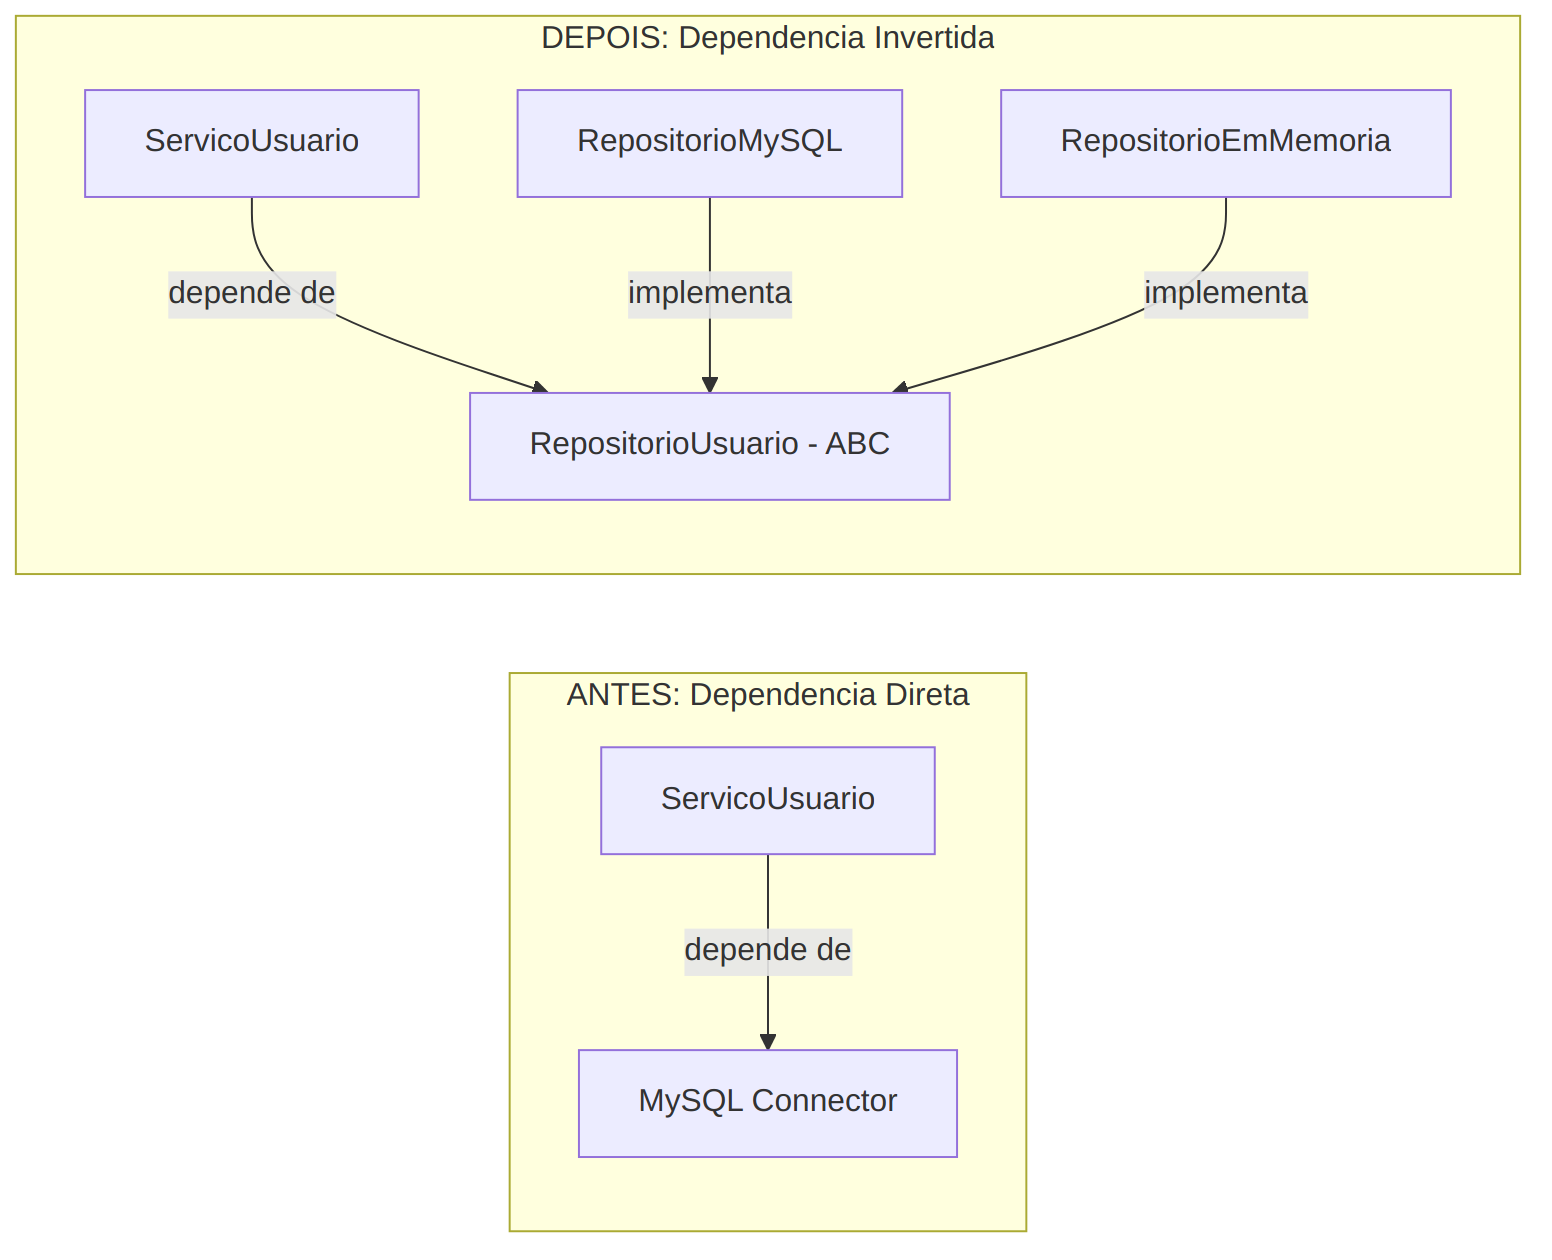
\includegraphics[width=0.85\textwidth]{imagens/03-principios-design-moderno-01-inversao-de-dependencia-antes-vs-depois-mermaid.png}
    \caption{Inversão de Dependência --- Antes vs Depois (Mermaid)}
\end{figure}


% ============================================================
\section{Além do SOLID}
% ============================================================

\subsection{KISS --- Keep It Simple, Stupid}

A solução mais simples que funciona é a melhor. Complexidade é inimiga número um
da manutenibilidade. Pergunte-se: ``Alguém que não conhece o contexto entenderia
este código em 30 segundos?'' Se não, simplifique.

\subsection{YAGNI --- You Ain't Gonna Need It}

Não construa para o futuro. Construa para o presente de forma extensível.
Generalização prematura é dívida técnica disfarçada de sofisticação. Antes de
adicionar uma abstração, pergunte: ``Existe um segundo caso de uso \emph{agora}?''

\subsection{DRY --- Don't Repeat Yourself}

Cada conhecimento tem uma única fonte. \textbf{Mas}: duplicação é melhor que a
abstração errada. Três repetições é um bom limiar para abstrair (a ``Regra de
Três''). Sandi Metz resume: ``Duplicação é muito mais barata que a abstração
errada.''

\subsection{Composition over Inheritance}

Prefira compor comportamentos a herdar classes. \texttt{TemMotor} e
\texttt{TemAsas} é melhor que \texttt{CarroVoador} estendendo \texttt{Veiculo}.

\begin{figure}[htbp]
    \centering
    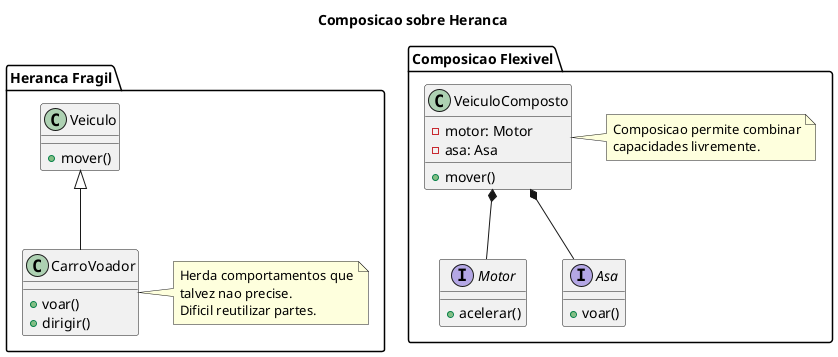
\includegraphics[width=0.85\textwidth]{imagens/03-principios-design-moderno-02-composicao-vs-heranca-plantuml.png}
    \caption{Composição vs Herança (PlantUML)}
\end{figure}

\begin{lstlisting}[language=Python, caption={Composição sobre Herança em Python}]
from abc import ABC, abstractmethod

# Capacidades como componentes
class Motor(ABC):
    @abstractmethod
    def acelerar(self) -> str: pass

class MotorEletrico(Motor):
    def acelerar(self) -> str:
        return "Acelerando silenciosamente..."

class MotorCombustao(Motor):
    def acelerar(self) -> str:
        return "Vrum vrum!"

class SistemaVoo(ABC):
    @abstractmethod
    def voar(self) -> str: pass

class AsaFixa(SistemaVoo):
    def voar(self) -> str:
        return "Planando com asas fixas..."

# Composicao: veiculos combinam capacidades
class Carro:
    def __init__(self, motor: Motor):
        self.motor = motor

    def mover(self) -> str:
        return self.motor.acelerar()

class CarroVoador:
    def __init__(self, motor: Motor, sistema_voo: SistemaVoo):
        self.motor = motor
        self.sistema_voo = sistema_voo

    def dirigir(self) -> str:
        return self.motor.acelerar()

    def voar(self) -> str:
        return self.sistema_voo.voar()

# Flexivel: qualquer combinacao e possivel
carro_eletrico = Carro(MotorEletrico())
carro_voador = CarroVoador(MotorCombustao(), AsaFixa())
\end{lstlisting}

\subsection{Princípio da Menor Surpresa}

Código deve se comportar como qualquer engenheiro razoável esperaria. Surpresas são
bugs. Um método chamado \texttt{obter\_usuario()} não deveria deletar registros como
efeito colateral. Um construtor não deveria fazer chamadas HTTP.


% ============================================================
\section{Clean Architecture e Ports \& Adapters}
% ============================================================

A Clean Architecture, proposta por Robert C. Martin, organiza o software em camadas
concêntricas onde a regra fundamental é: \textbf{dependências apontam para dentro}.
Camadas externas dependem de camadas internas, nunca o contrário.

\begin{figure}[htbp]
    \centering
    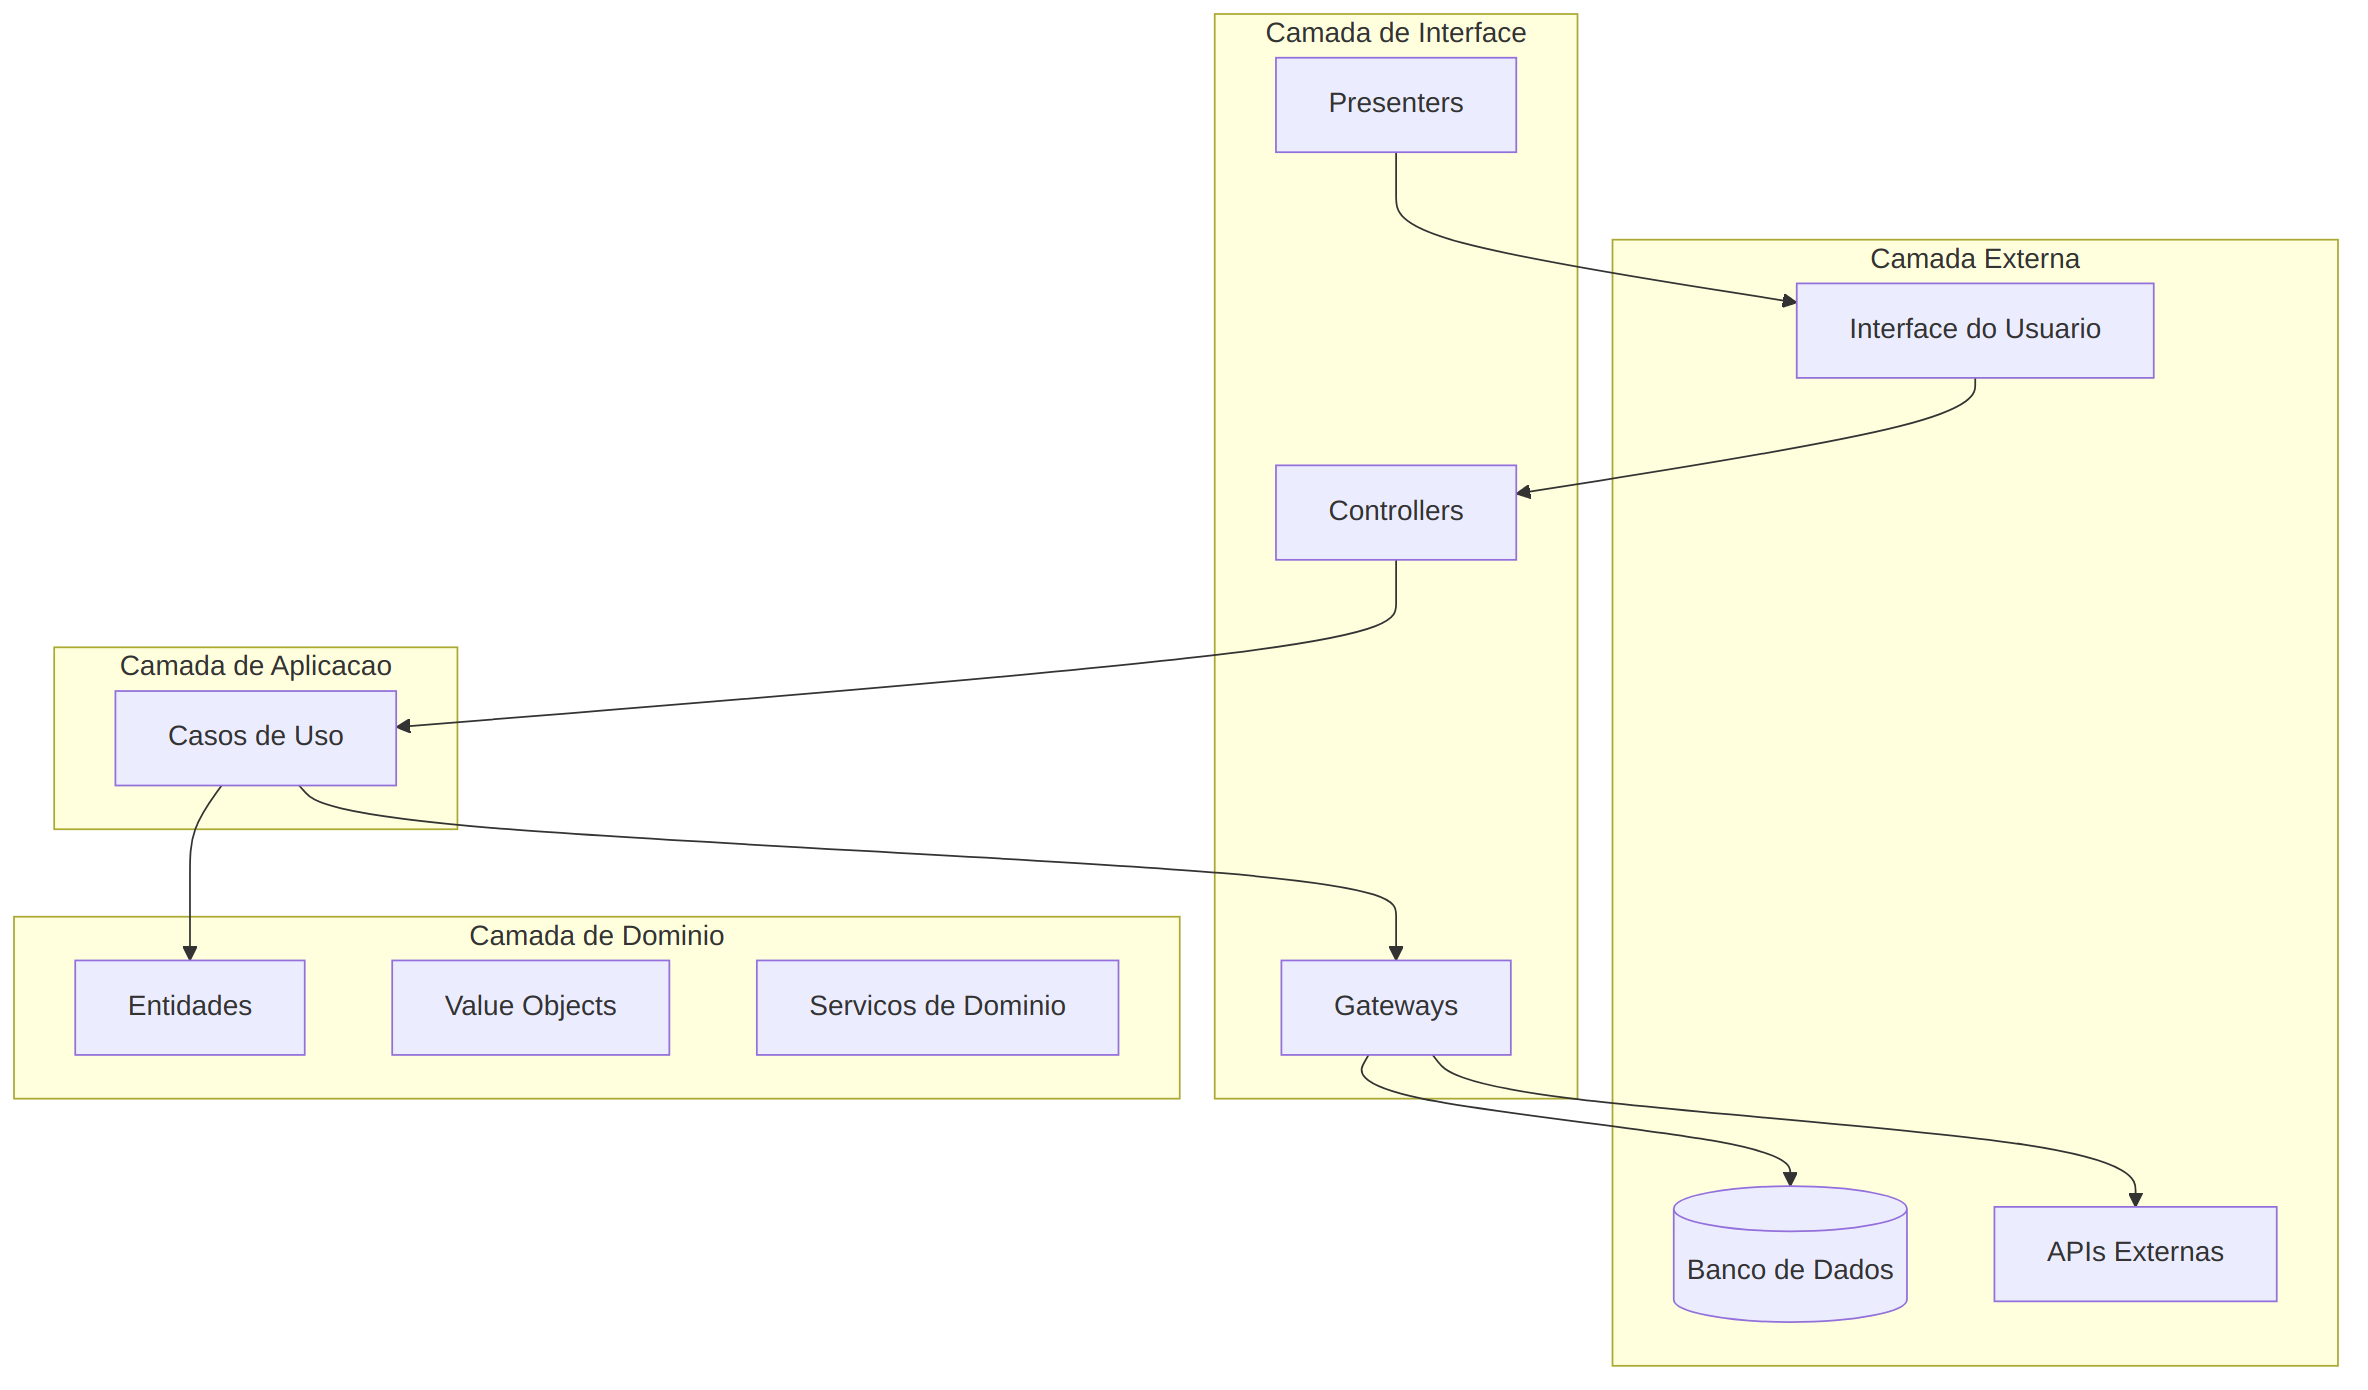
\includegraphics[width=0.85\textwidth]{imagens/03-principios-design-moderno-03-camadas-da-clean-architecture-mermaid.png}
    \caption{Camadas da Clean Architecture (Mermaid)}
\end{figure}

\subsection{As Quatro Camadas}

\begin{itemize}
    \item \textbf{Domínio}: entidades, value objects, regras de negócio puras. Não
    conhece banco de dados, HTTP, nem framework. É o coração do sistema.
    \item \textbf{Aplicação}: casos de uso que orquestram entidades. Define \emph{o
    que} o sistema faz, não \emph{como} persiste ou se comunica.
    \item \textbf{Interface}: controllers, presenters, view models. Traduz entre o
    mundo externo e a aplicação.
    \item \textbf{Infraestrutura}: banco de dados, APIs externas, filas, cache.
    Implementa as interfaces (ports) definidas pelo domínio.
\end{itemize}

\subsection{Regra de Ouro}

\textbf{O domínio não sabe que a web existe.} Se você remover toda a infraestrutura
(banco, HTTP, filas), o domínio continua compilando e seus testes continuam passando.
Essa é a prova de que a arquitetura está correta.

\subsection{Ports \& Adapters na Prática}

\begin{lstlisting}[language=Python, caption={Ports \& Adapters --- domínio define a porta, infraestrutura implementa}]
# === PORTA (definida no dominio) ===
from abc import ABC, abstractmethod
from dataclasses import dataclass
from datetime import datetime

@dataclass
class Transacao:
    id: str
    valor: float
    data: datetime
    descricao: str

class PortaTransacoes(ABC):
    """Porta definida pelo dominio. Infraestrutura implementa."""
    @abstractmethod
    def listar_por_periodo(
        self, inicio: datetime, fim: datetime
    ) -> list[Transacao]:
        pass

    @abstractmethod
    def salvar(self, transacao: Transacao) -> None:
        pass


# === CASO DE USO (camada de aplicacao) ===
class GerarExtrato:
    def __init__(self, repositorio: PortaTransacoes):
        self.repositorio = repositorio

    def executar(self, inicio: datetime, fim: datetime) -> dict:
        transacoes = self.repositorio.listar_por_periodo(inicio, fim)
        total = sum(t.valor for t in transacoes)
        return {
            "transacoes": transacoes,
            "total": total,
            "periodo": f"{inicio} a {fim}",
        }


# === ADAPTADOR (camada de infraestrutura) ===
class AdaptadorTransacoesPostgres(PortaTransacoes):
    def __init__(self, session):
        self.session = session

    def listar_por_periodo(
        self, inicio: datetime, fim: datetime
    ) -> list[Transacao]:
        rows = self.session.execute(
            "SELECT id, valor, data, descricao FROM transacoes "
            "WHERE data BETWEEN :inicio AND :fim",
            {"inicio": inicio, "fim": fim}
        ).fetchall()
        return [Transacao(*row) for row in rows]

    def salvar(self, transacao: Transacao) -> None:
        self.session.execute(
            "INSERT INTO transacoes VALUES (:id, :valor, :data, :desc)",
            {"id": transacao.id, "valor": transacao.valor,
             "data": transacao.data, "desc": transacao.descricao}
        )
        self.session.commit()
\end{lstlisting}


% ============================================================
\section{Design Patterns que Importam em 2025}
% ============================================================

Nem todo padrão do livro Gang of Four (GoF) é relevante no dia a dia moderno.
Alguns, porém, continuam indispensáveis. A tabela a seguir resume os padrões
mais úteis e quando aplicá-los.

\begin{table}[h!]
\centering
\caption{Design Patterns: Quando Usar}
\begin{tabular}{p{3cm} p{5cm} p{5cm}}
\toprule
\textbf{Padrão} & \textbf{Quando Usar} & \textbf{Quando Evitar} \\
\midrule
Strategy & Variações de algoritmo que mudam em runtime & Quando há apenas uma implementação fixa \\
Observer & Eventos desacoplados entre componentes & Quando a cadeia de eventos fica difícil de rastrear \\
Decorator & Adicionar comportamento sem alterar a classe & Quando a pilha de decoradores fica confusa \\
Repository & Isolar persistência do domínio & Em scripts simples ou CRUDs triviais \\
Factory & Criação complexa de objetos com variações & Quando \texttt{new Classe()} é suficiente \\
\bottomrule
\end{tabular}
\end{table}

\subsection{Strategy Pattern}

O padrão Strategy encapsula algoritmos intercambiáveis, permitindo que o cliente
escolha a implementação em tempo de execução.

\begin{figure}[htbp]
    \centering
    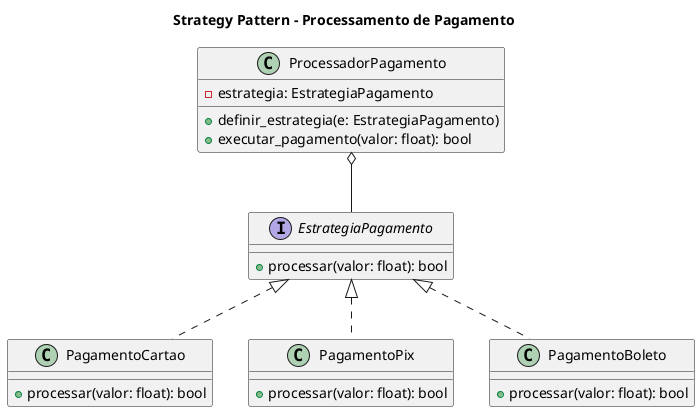
\includegraphics[width=0.85\textwidth]{imagens/03-principios-design-moderno-04-strategy-pattern-plantuml.png}
    \caption{Strategy Pattern (PlantUML)}
\end{figure}

\begin{lstlisting}[language=Python, caption={Strategy Pattern em Python}]
from abc import ABC, abstractmethod

class EstrategiaPagamento(ABC):
    @abstractmethod
    def processar(self, valor: float) -> bool:
        pass

class PagamentoCartao(EstrategiaPagamento):
    def processar(self, valor: float) -> bool:
        print(f"Processando R${valor} no cartao...")
        # Integra com gateway de cartao
        return True

class PagamentoPix(EstrategiaPagamento):
    def processar(self, valor: float) -> bool:
        print(f"Gerando QR Code Pix de R${valor}...")
        return True

class PagamentoBoleto(EstrategiaPagamento):
    def processar(self, valor: float) -> bool:
        print(f"Gerando boleto de R${valor}...")
        return True


class ProcessadorPagamento:
    def __init__(self, estrategia: EstrategiaPagamento):
        self.estrategia = estrategia

    def executar(self, valor: float) -> bool:
        return self.estrategia.processar(valor)

# Uso: trocar a estrategia sem alterar o processador
processador = ProcessadorPagamento(PagamentoPix())
processador.executar(150.00)
\end{lstlisting}

\subsection{Observer Pattern}

O Observer desacopla o emissor do evento dos interessados. Útil para notificações,
logs, e atualizações reativas.

\begin{lstlisting}[language=Python, caption={Observer Pattern em Python}]
from abc import ABC, abstractmethod

class Observador(ABC):
    @abstractmethod
    def atualizar(self, evento: str, dados: dict) -> None:
        pass

class EmissorEventos:
    def __init__(self):
        self._observadores: dict[str, list[Observador]] = {}

    def registrar(self, evento: str, observador: Observador):
        self._observadores.setdefault(evento, []).append(observador)

    def emitir(self, evento: str, dados: dict):
        for obs in self._observadores.get(evento, []):
            obs.atualizar(evento, dados)


# Observadores concretos
class LogObservador(Observador):
    def atualizar(self, evento: str, dados: dict) -> None:
        print(f"[LOG] Evento: {evento}, Dados: {dados}")

class EmailObservador(Observador):
    def atualizar(self, evento: str, dados: dict) -> None:
        print(f"[EMAIL] Notificando sobre: {evento}")

class MetricasObservador(Observador):
    def atualizar(self, evento: str, dados: dict) -> None:
        print(f"[METRICAS] Registrando: {evento}")


# Uso
emissor = EmissorEventos()
emissor.registrar("pedido_criado", LogObservador())
emissor.registrar("pedido_criado", EmailObservador())
emissor.registrar("pedido_criado", MetricasObservador())

emissor.emitir("pedido_criado", {"id": 42, "valor": 199.90})
\end{lstlisting}

\subsection{Decorator Pattern}

O Decorator adiciona comportamento a um objeto sem alterar sua interface. Perfeito
para cross-cutting concerns como cache, logging e retry.

\begin{lstlisting}[language=Python, caption={Decorator Pattern em Python}]
from abc import ABC, abstractmethod
import time

class ServicoClima(ABC):
    @abstractmethod
    def obter_temperatura(self, cidade: str) -> float:
        pass

class ServicoClimaReal(ServicoClima):
    def obter_temperatura(self, cidade: str) -> float:
        # Chamada real a API externa (lenta)
        time.sleep(2)
        return 25.0

class ServicoClimaComCache(ServicoClima):
    """Decorator: adiciona cache sem alterar o servico original."""
    def __init__(self, servico: ServicoClima, ttl: int = 300):
        self._servico = servico
        self._cache: dict = {}
        self._ttl = ttl

    def obter_temperatura(self, cidade: str) -> float:
        agora = time.time()
        if cidade in self._cache:
            valor, timestamp = self._cache[cidade]
            if agora - timestamp < self._ttl:
                print(f"[CACHE HIT] {cidade}")
                return valor

        print(f"[CACHE MISS] {cidade}")
        valor = self._servico.obter_temperatura(cidade)
        self._cache[cidade] = (valor, agora)
        return valor

class ServicoClimaComLog(ServicoClima):
    """Decorator: adiciona logging."""
    def __init__(self, servico: ServicoClima):
        self._servico = servico

    def obter_temperatura(self, cidade: str) -> float:
        print(f"[LOG] Consultando temperatura de {cidade}")
        resultado = self._servico.obter_temperatura(cidade)
        print(f"[LOG] Resultado: {resultado} graus C")
        return resultado


# Composicao de decorators
servico = ServicoClimaComLog(
    ServicoClimaComCache(
        ServicoClimaReal()
    )
)
temp = servico.obter_temperatura("Sao Paulo")
\end{lstlisting}

\subsection{Repository Pattern}

Já demonstrado na seção de DIP. O Repository isola a lógica de persistência do
domínio, permitindo trocar a implementação (banco relacional, NoSQL, memória)
sem afetar as regras de negócio.

\subsection{Factory Pattern}

O Factory encapsula a complexidade de criação de objetos, especialmente quando
a lógica de instanciação envolve condições ou configurações.

\begin{lstlisting}[language=Python, caption={Factory Pattern em Python}]
from dataclasses import dataclass

@dataclass
class ConexaoBanco:
    host: str
    porta: int
    driver: str

class FabricaConexao:
    """Factory: encapsula a logica de criacao complexa."""

    @staticmethod
    def criar(tipo: str, config: dict) -> ConexaoBanco:
        fabricas = {
            "postgres": lambda c: ConexaoBanco(
                host=c.get("host", "localhost"),
                porta=c.get("porta", 5432),
                driver="psycopg2"
            ),
            "mysql": lambda c: ConexaoBanco(
                host=c.get("host", "localhost"),
                porta=c.get("porta", 3306),
                driver="mysql-connector"
            ),
            "sqlite": lambda c: ConexaoBanco(
                host=c.get("caminho", ":memory:"),
                porta=0,
                driver="sqlite3"
            ),
        }

        fabrica = fabricas.get(tipo)
        if not fabrica:
            raise ValueError(f"Tipo de banco desconhecido: {tipo}")
        return fabrica(config)


# Uso
conexao = FabricaConexao.criar("postgres", {"host": "db.empresa.com"})
\end{lstlisting}


% ============================================================
\section{Anti-padrões e Code Smells}
% ============================================================

Anti-padrões são soluções recorrentes que parecem boas mas geram problemas. Code
smells são sintomas --- indicadores de que algo pode estar errado no design.

\subsection{Anti-padrões Comuns}

\subsubsection{God Class (Classe Deus)}

Uma classe que faz tudo: valida, persiste, notifica, formata, calcula. Viola
SRP de forma grotesca.

\begin{lstlisting}[language=Python, caption={Anti-padrão: God Class}]
class SistemaCompleto:
    """Esta classe faz TUDO. Nao faca isso."""
    def autenticar_usuario(self, login, senha): ...
    def criar_pedido(self, itens): ...
    def processar_pagamento(self, valor): ...
    def enviar_email(self, destinatario, corpo): ...
    def gerar_relatorio_pdf(self, dados): ...
    def sincronizar_estoque(self): ...
    def fazer_backup(self): ...
    # 2000 linhas depois...
\end{lstlisting}

\textbf{Solução}: Extrair classes por responsabilidade. Cada domínio funcional
vira um serviço próprio.

\subsubsection{Shotgun Surgery (Cirurgia de Espingarda)}

Uma única mudança de negócio exige alterar 15 arquivos diferentes. Sinal de que
a responsabilidade está espalhada.

\textbf{Solução}: Consolidar a lógica relacionada em um único módulo.

\subsubsection{Feature Envy (Inveja de Funcionalidade)}

Um método que usa mais dados de outra classe do que da própria.

\begin{lstlisting}[language=Python, caption={Code Smell: Feature Envy}]
# RUIM: metodo de Relatorio usando dados internos de Pedido
class Relatorio:
    def calcular_total_pedido(self, pedido):
        total = 0
        for item in pedido.itens:  # acessando internals do Pedido
            total += item.preco * item.quantidade
            if pedido.cliente.tipo == "vip":
                total *= 0.9
        return total

# BOM: mover a logica para onde os dados estao
class Pedido:
    def calcular_total(self) -> float:
        subtotal = sum(i.preco * i.quantidade for i in self.itens)
        if self.cliente.tipo == "vip":
            return subtotal * 0.9
        return subtotal
\end{lstlisting}

\subsubsection{Primitive Obsession (Obsessão por Primitivos)}

Usar strings e inteiros onde Value Objects seriam mais expressivos e seguros.

\begin{lstlisting}[language=Python, caption={Code Smell: Primitive Obsession vs Value Objects}]
# RUIM: tudo e string
def criar_usuario(nome: str, email: str, cpf: str, telefone: str):
    # Nenhuma validacao no tipo. Email e CPF sao apenas strings.
    pass

# BOM: Value Objects com validacao embutida
@dataclass(frozen=True)
class Email:
    valor: str
    def __post_init__(self):
        if "@" not in self.valor:
            raise ValueError(f"Email invalido: {self.valor}")

@dataclass(frozen=True)
class CPF:
    valor: str
    def __post_init__(self):
        digitos = self.valor.replace(".", "").replace("-", "")
        if len(digitos) != 11:
            raise ValueError(f"CPF invalido: {self.valor}")

def criar_usuario(nome: str, email: Email, cpf: CPF):
    # Agora o sistema de tipos garante validade
    pass
\end{lstlisting}

\subsubsection{Outros Code Smells Importantes}

\begin{itemize}
    \item \textbf{Long Method}: métodos com mais de 20 linhas geralmente fazem
    coisas demais. Extraia sub-métodos com nomes descritivos.
    \item \textbf{Deep Nesting}: mais de 3 níveis de indentação são difíceis de
    ler. Use early returns e extraia funções.
    \item \textbf{Boolean Parameters}: \texttt{processar(pedido, True, False, True)}
    é ilegível. Use enums ou objetos de configuração.
    \item \textbf{Magic Numbers}: \texttt{if dias > 30} --- o que é 30? Use
    constantes nomeadas: \texttt{PRAZO\_MAXIMO\_DIAS = 30}.
    \item \textbf{Dead Code}: código comentado ou inalcançável. Delete-o. O
    controle de versão guarda o histórico.
\end{itemize}


% ============================================================
\section{Catálogo de Técnicas de Refatoração}
% ============================================================

Refatorar é alterar a estrutura interna do código sem mudar seu comportamento
externo. A seguir, as técnicas mais importantes.

\subsection{Extract Method (Extrair Método)}

Quando um trecho de código pode ser agrupado e nomeado.

\begin{lstlisting}[language=Python, caption={Refatoração: Extract Method}]
# ANTES: metodo longo e confuso
def processar_pedido(pedido):
    # Validacao
    if not pedido.itens:
        raise ValueError("Pedido vazio")
    if not pedido.cliente:
        raise ValueError("Cliente ausente")
    for item in pedido.itens:
        if item.quantidade <= 0:
            raise ValueError(f"Quantidade invalida: {item}")

    # Calculo
    subtotal = sum(i.preco * i.quantidade for i in pedido.itens)
    imposto = subtotal * 0.15
    total = subtotal + imposto

    # Persistencia
    db.salvar(pedido, total)
    return total


# DEPOIS: metodos extraidos com nomes claros
def processar_pedido(pedido):
    validar_pedido(pedido)
    total = calcular_total_com_imposto(pedido)
    db.salvar(pedido, total)
    return total

def validar_pedido(pedido):
    if not pedido.itens:
        raise ValueError("Pedido vazio")
    if not pedido.cliente:
        raise ValueError("Cliente ausente")
    for item in pedido.itens:
        if item.quantidade <= 0:
            raise ValueError(f"Quantidade invalida: {item}")

def calcular_total_com_imposto(pedido, taxa_imposto=0.15):
    subtotal = sum(i.preco * i.quantidade for i in pedido.itens)
    return subtotal * (1 + taxa_imposto)
\end{lstlisting}

\subsection{Replace Conditional with Polymorphism}

Substituir cadeias de \texttt{if/elif} por polimorfismo (já demonstrado no OCP).

\subsection{Introduce Parameter Object}

Quando uma função recebe muitos parâmetros relacionados, agrupe-os.

\begin{lstlisting}[language=Python, caption={Refatoração: Introduce Parameter Object}]
# ANTES: muitos parametros soltos
def buscar_transacoes(
    data_inicio, data_fim, valor_min, valor_max,
    tipo, status, cliente_id, limite, pagina
):
    ...

# DEPOIS: parametros agrupados em objeto
@dataclass
class FiltroTransacoes:
    data_inicio: datetime
    data_fim: datetime
    valor_min: float = 0
    valor_max: float = float("inf")
    tipo: str | None = None
    status: str | None = None
    cliente_id: int | None = None
    limite: int = 50
    pagina: int = 1

def buscar_transacoes(filtro: FiltroTransacoes):
    ...
\end{lstlisting}

\subsection{Replace Inheritance with Delegation}

Quando a herança cria acoplamento indesejado, substitua por composição/delegação
(já demonstrado em ``Composition over Inheritance'').

\subsection{Guard Clauses (Cláusulas de Guarda)}

Eliminar aninhamento profundo com retornos antecipados.

\begin{lstlisting}[language=Python, caption={Refatoração: Guard Clauses}]
# ANTES: deep nesting
def calcular_desconto(pedido):
    if pedido is not None:
        if pedido.cliente is not None:
            if pedido.cliente.ativo:
                if pedido.valor > 100:
                    return pedido.valor * 0.1
                else:
                    return 0
            else:
                return 0
        else:
            return 0
    else:
        return 0

# DEPOIS: guard clauses
def calcular_desconto(pedido):
    if pedido is None:
        return 0
    if pedido.cliente is None:
        return 0
    if not pedido.cliente.ativo:
        return 0
    if pedido.valor <= 100:
        return 0
    return pedido.valor * 0.1
\end{lstlisting}


% ============================================================
\section{Design Funcional}
% ============================================================

Princípios da programação funcional melhoram código em qualquer paradigma. Não é
preciso usar Haskell para se beneficiar de imutabilidade, funções puras e
composição.

\subsection{Imutabilidade}

Dados que não mudam são mais fáceis de raciocinar. \texttt{const} por padrão,
\texttt{let} por exceção. Em Python, use \texttt{@dataclass(frozen=True)},
\texttt{tuple} em vez de \texttt{list}, e \texttt{frozenset} quando possível.

\begin{lstlisting}[language=Python, caption={Imutabilidade em Python}]
from dataclasses import dataclass

# MUTAVEL: perigoso em contextos concorrentes
class ContaMutavel:
    def __init__(self, saldo: float):
        self.saldo = saldo

    def depositar(self, valor: float):
        self.saldo += valor  # Modifica o estado

# IMUTAVEL: seguro e previsivel
@dataclass(frozen=True)
class ContaImutavel:
    saldo: float

    def depositar(self, valor: float) -> "ContaImutavel":
        # Retorna NOVA instancia em vez de modificar
        return ContaImutavel(saldo=self.saldo + valor)

conta = ContaImutavel(saldo=1000)
conta_nova = conta.depositar(500)
print(conta.saldo)       # 1000 (original intacta)
print(conta_nova.saldo)  # 1500
\end{lstlisting}

\subsection{Funções Puras}

Mesma entrada = mesma saída, sem efeitos colaterais. Fáceis de testar, compor,
paralelizar e cachear.

\begin{lstlisting}[language=Python, caption={Funções puras vs impuras}]
# IMPURA: depende de estado externo
taxa_global = 0.15

def calcular_imposto_impuro(valor):
    return valor * taxa_global  # Resultado muda se taxa_global mudar

# PURA: tudo explicito nos parametros
def calcular_imposto_puro(valor: float, taxa: float) -> float:
    return valor * taxa  # Sempre o mesmo resultado para mesma entrada
\end{lstlisting}

\subsection{Efeitos Colaterais Controlados}

IO, banco de dados, rede --- isolados em camadas específicas. O núcleo é puro.
Padrão Functional Core, Imperative Shell.

\subsection{Option/Maybe e Either}

Substituem \texttt{null} e exceções por tipos que forçam tratamento explícito.
Em Python, use \texttt{Optional} e \texttt{Result} (bibliotecas como \texttt{returns}).


% ============================================================
\section{Design para Testabilidade}
% ============================================================

Código testável é código bem desenhado. Se é difícil testar, o design está
pedindo ajuda.

\subsection{Injeção de Dependência}

Não crie dependências dentro do construtor. Receba-as.

\begin{lstlisting}[language=Python, caption={Injeção de Dependência para testabilidade}]
# DIFICIL DE TESTAR: cria dependencias internamente
class ServicoRelatorio:
    def __init__(self):
        self.banco = ConexaoPostgres()  # Acoplado!
        self.email = ServicoSMTP()       # Acoplado!

    def gerar_e_enviar(self, mes: int):
        dados = self.banco.buscar_vendas(mes)
        # ... gera relatorio ...
        self.email.enviar(relatorio)


# FACIL DE TESTAR: recebe dependencias
class ServicoRelatorio:
    def __init__(self, repositorio: RepositorioVendas,
                 notificador: Notificador):
        self.repositorio = repositorio
        self.notificador = notificador

    def gerar_e_enviar(self, mes: int):
        dados = self.repositorio.buscar_vendas(mes)
        # ... gera relatorio ...
        self.notificador.enviar(relatorio)


# No teste: injetar mocks
def test_gerar_relatorio():
    repo_mock = RepositorioEmMemoria(vendas=[Venda(100), Venda(200)])
    notificador_mock = NotificadorFalso()

    servico = ServicoRelatorio(repo_mock, notificador_mock)
    servico.gerar_e_enviar(mes=3)

    assert notificador_mock.enviados == 1
\end{lstlisting}

\subsection{Mocks e Stubs como Feedback de Design}

Se é difícil mockar uma dependência, o acoplamento está alto. Mocks dolorosos são
sintomas, não o problema. O problema é o design.

\subsection{Testabilidade como Métrica}

Se você não consegue testar uma função em isolamento, ela faz coisas demais. A
dificuldade de testar é o melhor \emph{code smell} que existe.

\subsection{Efeito Colateral Visível}

Funções que retornam valores em vez de modificar estado global são naturalmente
testáveis. Prefira retornar resultados a modificar parâmetros por referência.


% ============================================================
\section{Como a IA Aplica Esses Princípios (e Quando Erra)}
% ============================================================

Ferramentas de IA como GitHub Copilot, ChatGPT e Claude são treinadas em bilhões
de linhas de código --- incluindo código ruim. Isso gera padrões previsíveis de
acerto e erro.

\subsection{Quando a IA Acerta}

\begin{itemize}
    \item \textbf{Padrões bem estabelecidos}: a IA gera Repository, Factory e
    Strategy com competência quando o contexto é claro.
    \item \textbf{Boilerplate}: código repetitivo como getters, setters,
    serialização e validação básica.
    \item \textbf{Testes unitários simples}: dado um método puro, a IA gera
    testes com boa cobertura de casos.
    \item \textbf{Refatorações mecânicas}: renomear variáveis, extrair métodos,
    converter loops para list comprehensions.
\end{itemize}

\subsection{Quando a IA Erra}

\begin{itemize}
    \item \textbf{God Class por acumulação}: ao pedir ``adicione funcionalidade X'',
    a IA tende a enfiar tudo na classe existente em vez de criar novas classes.
    Ela otimiza para \emph{localidade} (mínima mudança), não para \emph{design}.
    \item \textbf{Abstrações prematuras}: a IA pode criar interfaces e factories
    para código que tem uma única implementação, violando YAGNI.
    \item \textbf{Dependências concretas}: sem instrução explícita, a IA frequentemente
    gera código acoplado a implementações específicas (violando DIP).
    \item \textbf{Ignorância do contexto arquitetural}: a IA não sabe em qual camada
    da Clean Architecture o código deveria estar. Ela coloca lógica de banco no
    domínio sem perceber.
    \item \textbf{Nomes genéricos}: \texttt{Manager}, \texttt{Handler},
    \texttt{Utils}, \texttt{Helper} --- nomes que não comunicam responsabilidade.
\end{itemize}

\subsection{Estratégias para Guiar a IA}

\begin{enumerate}
    \item \textbf{Forneça contexto arquitetural}: inclua no prompt a estrutura de
    camadas e onde o código deve ficar.
    \item \textbf{Peça explicitamente}: ``Aplique SRP'' ou ``Use injeção de
    dependência'' no prompt.
    \item \textbf{Revise o resultado}: trate código gerado por IA como código de
    um junior talentoso --- funciona, mas precisa de revisão de design.
    \item \textbf{Use testes como contrato}: se você tem testes, a IA pode gerar
    código que os satisfaça sem violar a arquitetura.
\end{enumerate}


% ============================================================
\section{Princípios em Conflito}
% ============================================================

Na teoria, princípios se complementam. Na prática, eles frequentemente entram em
conflito. O engenheiro maduro reconhece o conflito e faz uma escolha consciente,
documentando o \emph{trade-off}.

\subsection{SOLID vs KISS}

Aplicar todos os princípios SOLID a um CRUD simples gera sobre-engenharia.
Uma classe com interface, implementação, factory e injeção de dependência para
um serviço que só faz \texttt{salvar()} e \texttt{buscar()} é complexidade
acidental.

\textbf{Heurística}: aplique SOLID quando houver variação real ou quando o código
será modificado por múltiplas pessoas. Para scripts, protótipos e código descartável,
KISS prevalece.

\subsection{DRY vs Acoplamento}

Eliminar duplicação às vezes cria acoplamento entre módulos que deveriam ser
independentes. Dois microsserviços com lógica semelhante não devem compartilhar
uma biblioteca se isso cria uma dependência de deploy entre eles.

\textbf{Heurística}: DRY dentro de um módulo, duplicação tolerada entre módulos
que escalam independentemente.

\subsection{YAGNI vs OCP}

YAGNI diz ``não construa para o futuro''. OCP diz ``projete para extensão''.
Como conciliar?

\textbf{Heurística}: não crie a abstração até precisar, mas quando criar, projete-a
para ser extensível. A primeira implementação pode ser concreta. Quando surgir o
segundo caso, refatore para abstração.

\subsection{SRP vs Praticidade}

Levar o SRP ao extremo gera classes com um único método e centenas de arquivos
minúsculos. O código fica ``bem projetado'' mas impossível de navegar.

\textbf{Heurística}: SRP se aplica a \emph{razões para mudar}, não a
\emph{quantidade de métodos}. Uma classe com cinco métodos que mudam pela mesma
razão está perfeitamente aderente ao SRP.

\subsection{Tabela de Decisão}

\begin{table}[h!]
\centering
\caption{Complexidade Acidental vs Essencial}
\begin{tabular}{p{3.5cm} p{4.5cm} p{4.5cm}}
\toprule
\textbf{Situação} & \textbf{Complexidade Acidental} & \textbf{Complexidade Essencial} \\
\midrule
Abstração sem segundo caso de uso & Factory para classe única & Cálculo tributário com 27 estados \\
Framework para 3 telas & Microsserviços para TODO app & Motor de regras de crédito \\
Otimização prematura & Cache em memória para 10 registros & Cache para API com 1M req/s \\
Generalização & \texttt{AbstractSingletonProxyFactory} & Interface \texttt{Repositorio} com 2+ implementações \\
\bottomrule
\end{tabular}
\end{table}


% ============================================================
\section{Simplicidade Intencional}
% ============================================================

Simplicidade não é ausência de complexidade --- é complexidade \textbf{gerenciada}.

\subsection{Complexidade Acidental vs Essencial}

\begin{itemize}
    \item \textbf{Complexidade acidental}: vem de más decisões, acoplamento, falta
    de clareza. Deve ser removida impiedosamente.
    \item \textbf{Complexidade essencial}: vem do problema real. Deve ser
    encapsulada em módulos com interfaces claras.
\end{itemize}

A pergunta-chave é: ``Esta complexidade existe por causa do \emph{problema} ou por
causa da \emph{solução}?''

\subsection{Refatoração como Ferramenta de Simplificação}

Código deve ficar mais simples com o tempo, não mais complexo --- se alguém cuidar
disso. Refatoração contínua é higiene, não luxo.

\subsection{O Corajoso Ato de Deletar Código}

Cada linha removida é uma linha que não precisa ser lida, testada, debugada e
mantida. Código comentado é código morto. Delete-o. O Git guarda o histórico.

\textbf{Regra prática}: se você pode remover código sem mudar comportamento
observável, esse código nunca deveria ter estado lá.

\subsection{Métricas de Simplicidade}

\begin{itemize}
    \item \textbf{Complexidade ciclomática}: número de caminhos independentes no
    código. Acima de 10, considere refatorar.
    \item \textbf{Profundidade de aninhamento}: mais de 3 níveis = extraia funções.
    \item \textbf{Número de parâmetros}: mais de 3 = considere Parameter Object.
    \item \textbf{Tamanho da classe}: acima de 200 linhas, investigue se há
    responsabilidades escondidas.
    \item \textbf{Tamanho do método}: acima de 20 linhas, considere Extract Method.
\end{itemize}


% ============================================================
\section{Conclusão}
% ============================================================

Princípios são ferramentas de pensamento. Use-os com discernimento, não com
fanatismo. O bom engenheiro sabe quando seguir e quando quebrar a regra ---
e, mais importante, sabe \emph{explicar por quê}.

Os princípios que discutimos neste capítulo --- SOLID, KISS, YAGNI, DRY,
composição sobre herança, Clean Architecture --- não são fins em si mesmos. São
meios para atingir código que:

\begin{enumerate}
    \item \textbf{Funciona corretamente} --- satisfaz os requisitos.
    \item \textbf{É compreensível} --- outro engenheiro consegue entender.
    \item \textbf{É modificável} --- mudanças são localizadas e seguras.
    \item \textbf{É testável} --- comportamento pode ser verificado automaticamente.
\end{enumerate}

Na era da IA, esses princípios são mais importantes do que nunca. A IA gera código
rápido. O engenheiro garante que esse código é \emph{bom}. A velocidade sem
princípios produz débito técnico na velocidade da luz.


% ============================================================
\section*{Exercícios}
% ============================================================

\begin{enumerate}
    \item Identifique uma violação do Open/Closed Principle em um código existente.
    Proponha uma refatoração usando Strategy Pattern.

    \item Refatore um trecho de código aplicando Composition over Inheritance.
    Compare a clareza das duas abordagens.

    \item Discuta: em que situações violar DRY é a decisão correta? Dê exemplos
    concretos de quando a duplicação é preferível à abstração.

    \item Pegue uma God Class de um projeto real (ou peça à IA para gerar uma).
    Aplique SRP para dividi-la em classes coesas. Quantas classes resultaram?

    \item Crie um exemplo de Decorator Pattern que adicione logging e retry a um
    serviço HTTP. Demonstre como os decorators podem ser compostos.

    \item Peça a uma IA para gerar um módulo de autenticação. Revise o resultado
    e identifique pelo menos 3 violações de princípios discutidos neste capítulo.
    Proponha as correções.

    \item Encontre uma situação real onde SOLID conflita com KISS. Documente o
    trade-off e justifique qual princípio você priorizaria e por quê.

    \item Aplique Guard Clauses a um método com mais de 3 níveis de aninhamento.
    Compare a legibilidade antes e depois.
\end{enumerate}
